\documentclass[ignorenonframetext,]{beamer}
\setbeamertemplate{caption}[numbered]
\setbeamertemplate{caption label separator}{: }
\setbeamercolor{caption name}{fg=normal text.fg}
\beamertemplatenavigationsymbolsempty
\usepackage{lmodern}
\usepackage{amssymb,amsmath}
\usepackage{ifxetex,ifluatex}
\usepackage{fixltx2e} % provides \textsubscript
\ifnum 0\ifxetex 1\fi\ifluatex 1\fi=0 % if pdftex
  \usepackage[T1]{fontenc}
  \usepackage[utf8]{inputenc}
\else % if luatex or xelatex
  \ifxetex
    \usepackage{mathspec}
  \else
    \usepackage{fontspec}
  \fi
  \defaultfontfeatures{Ligatures=TeX,Scale=MatchLowercase}
\fi
\usefonttheme{structurebold}
% use upquote if available, for straight quotes in verbatim environments
\IfFileExists{upquote.sty}{\usepackage{upquote}}{}
% use microtype if available
\IfFileExists{microtype.sty}{%
\usepackage{microtype}
\UseMicrotypeSet[protrusion]{basicmath} % disable protrusion for tt fonts
}{}
\newif\ifbibliography
\usepackage{color}
\usepackage{fancyvrb}
\newcommand{\VerbBar}{|}
\newcommand{\VERB}{\Verb[commandchars=\\\{\}]}
\DefineVerbatimEnvironment{Highlighting}{Verbatim}{commandchars=\\\{\}}
% Add ',fontsize=\small' for more characters per line
\usepackage{framed}
\definecolor{shadecolor}{RGB}{248,248,248}
\newenvironment{Shaded}{\begin{snugshade}}{\end{snugshade}}
\newcommand{\KeywordTok}[1]{\textcolor[rgb]{0.13,0.29,0.53}{\textbf{{#1}}}}
\newcommand{\DataTypeTok}[1]{\textcolor[rgb]{0.13,0.29,0.53}{{#1}}}
\newcommand{\DecValTok}[1]{\textcolor[rgb]{0.00,0.00,0.81}{{#1}}}
\newcommand{\BaseNTok}[1]{\textcolor[rgb]{0.00,0.00,0.81}{{#1}}}
\newcommand{\FloatTok}[1]{\textcolor[rgb]{0.00,0.00,0.81}{{#1}}}
\newcommand{\ConstantTok}[1]{\textcolor[rgb]{0.00,0.00,0.00}{{#1}}}
\newcommand{\CharTok}[1]{\textcolor[rgb]{0.31,0.60,0.02}{{#1}}}
\newcommand{\SpecialCharTok}[1]{\textcolor[rgb]{0.00,0.00,0.00}{{#1}}}
\newcommand{\StringTok}[1]{\textcolor[rgb]{0.31,0.60,0.02}{{#1}}}
\newcommand{\VerbatimStringTok}[1]{\textcolor[rgb]{0.31,0.60,0.02}{{#1}}}
\newcommand{\SpecialStringTok}[1]{\textcolor[rgb]{0.31,0.60,0.02}{{#1}}}
\newcommand{\ImportTok}[1]{{#1}}
\newcommand{\CommentTok}[1]{\textcolor[rgb]{0.56,0.35,0.01}{\textit{{#1}}}}
\newcommand{\DocumentationTok}[1]{\textcolor[rgb]{0.56,0.35,0.01}{\textbf{\textit{{#1}}}}}
\newcommand{\AnnotationTok}[1]{\textcolor[rgb]{0.56,0.35,0.01}{\textbf{\textit{{#1}}}}}
\newcommand{\CommentVarTok}[1]{\textcolor[rgb]{0.56,0.35,0.01}{\textbf{\textit{{#1}}}}}
\newcommand{\OtherTok}[1]{\textcolor[rgb]{0.56,0.35,0.01}{{#1}}}
\newcommand{\FunctionTok}[1]{\textcolor[rgb]{0.00,0.00,0.00}{{#1}}}
\newcommand{\VariableTok}[1]{\textcolor[rgb]{0.00,0.00,0.00}{{#1}}}
\newcommand{\ControlFlowTok}[1]{\textcolor[rgb]{0.13,0.29,0.53}{\textbf{{#1}}}}
\newcommand{\OperatorTok}[1]{\textcolor[rgb]{0.81,0.36,0.00}{\textbf{{#1}}}}
\newcommand{\BuiltInTok}[1]{{#1}}
\newcommand{\ExtensionTok}[1]{{#1}}
\newcommand{\PreprocessorTok}[1]{\textcolor[rgb]{0.56,0.35,0.01}{\textit{{#1}}}}
\newcommand{\AttributeTok}[1]{\textcolor[rgb]{0.77,0.63,0.00}{{#1}}}
\newcommand{\RegionMarkerTok}[1]{{#1}}
\newcommand{\InformationTok}[1]{\textcolor[rgb]{0.56,0.35,0.01}{\textbf{\textit{{#1}}}}}
\newcommand{\WarningTok}[1]{\textcolor[rgb]{0.56,0.35,0.01}{\textbf{\textit{{#1}}}}}
\newcommand{\AlertTok}[1]{\textcolor[rgb]{0.94,0.16,0.16}{{#1}}}
\newcommand{\ErrorTok}[1]{\textcolor[rgb]{0.64,0.00,0.00}{\textbf{{#1}}}}
\newcommand{\NormalTok}[1]{{#1}}
\usepackage{graphicx,grffile}
\makeatletter
\def\maxwidth{\ifdim\Gin@nat@width>\linewidth\linewidth\else\Gin@nat@width\fi}
\def\maxheight{\ifdim\Gin@nat@height>\textheight0.8\textheight\else\Gin@nat@height\fi}
\makeatother
% Scale images if necessary, so that they will not overflow the page
% margins by default, and it is still possible to overwrite the defaults
% using explicit options in \includegraphics[width, height, ...]{}
\setkeys{Gin}{width=\maxwidth,height=\maxheight,keepaspectratio}

% Prevent slide breaks in the middle of a paragraph:
\widowpenalties 1 10000
\raggedbottom

\AtBeginPart{
  \let\insertpartnumber\relax
  \let\partname\relax
  \frame{\partpage}
}
\AtBeginSection{
  \ifbibliography
  \else
    \let\insertsectionnumber\relax
    \let\sectionname\relax
    \frame{\sectionpage}
  \fi
}
\AtBeginSubsection{
  \let\insertsubsectionnumber\relax
  \let\subsectionname\relax
  \frame{\subsectionpage}
}

\setlength{\emergencystretch}{3em}  % prevent overfull lines
\providecommand{\tightlist}{%
  \setlength{\itemsep}{0pt}\setlength{\parskip}{0pt}}
\setcounter{secnumdepth}{0}
\definecolor{links}{HTML}{800080}
\hypersetup{colorlinks,linkcolor=,urlcolor=links}

\title{Web Data Collection with R}
\subtitle{HTML Forms POST Case Study}
\author{Peter Meißner / 2016-02-29 -- 2016-03-04 / ECPR WSMT}
\date{}

\begin{document}
\frame{\titlepage}

\begin{frame}
\tableofcontents[hideallsubsections]
\end{frame}

\section{Posting HTML Forms}\label{posting-html-forms}

\begin{frame}{Teaser}

\begin{itemize}
\tightlist
\item
  ADCR author blog post on \url{http://www.r-datacollection.com/} battle
  against each other for the readability price
\end{itemize}

\end{frame}

\begin{frame}[fragile]{a first glance}

\begin{Shaded}
\begin{Highlighting}[]
\CommentTok{# ADCR: page 236}
\NormalTok{attr_inspector <-}\StringTok{ }\NormalTok{function(parsed_html, xpath)\{}
  \NormalTok{x <-}\StringTok{ }\KeywordTok{html_nodes}\NormalTok{(parsed_html, }\DataTypeTok{xpath=}\NormalTok{xpath)}
  \NormalTok{x <-}\StringTok{ }\KeywordTok{html_attrs}\NormalTok{(x)}
  \NormalTok{x <-}\StringTok{ }\KeywordTok{lapply}\NormalTok{(x, function(x) }\KeywordTok{as.data.frame}\NormalTok{(}\KeywordTok{t}\NormalTok{(x)) )}
  \KeywordTok{do.call}\NormalTok{(plyr::rbind.fill, x)}
\NormalTok{\}}
\end{Highlighting}
\end{Shaded}

\begin{Shaded}
\begin{Highlighting}[]
\KeywordTok{library}\NormalTok{(httr)}
\KeywordTok{library}\NormalTok{(rvest)}
\end{Highlighting}
\end{Shaded}

\begin{verbatim}
## Loading required package: xml2
\end{verbatim}

\begin{Shaded}
\begin{Highlighting}[]
\KeywordTok{library}\NormalTok{(stringr)}
\end{Highlighting}
\end{Shaded}

\end{frame}

\begin{frame}[fragile]{a first glance}

\begin{Shaded}
\begin{Highlighting}[]
\NormalTok{url  <-}\StringTok{ "http://read-able.com/"}
\NormalTok{html <-}\StringTok{ }\KeywordTok{read_html}\NormalTok{(url)}
\KeywordTok{attr_inspector}\NormalTok{( html, }\StringTok{"//form"}\NormalTok{)}
\end{Highlighting}
\end{Shaded}

\begin{verbatim}
##   method    action
## 1    get check.php
## 2   post check.php
\end{verbatim}

\begin{Shaded}
\begin{Highlighting}[]
\KeywordTok{attr_inspector}\NormalTok{( html, }\StringTok{"//form[2]//input|//textarea|//select"}\NormalTok{)}
\end{Highlighting}
\end{Shaded}

\begin{verbatim}
##            id        name rows cols
## 1 directInput directInput   10   60
\end{verbatim}

\end{frame}

\begin{frame}{HTTP messages}

\begin{itemize}
\tightlist
\item
  but where goes our data?
\end{itemize}

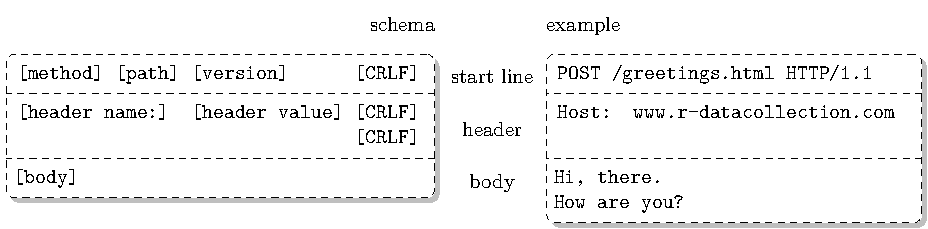
\includegraphics{fig/httprequest.pdf}

\end{frame}

\begin{frame}{HTTP messages}

\begin{itemize}
\tightlist
\item
  but where goes our data?
\end{itemize}

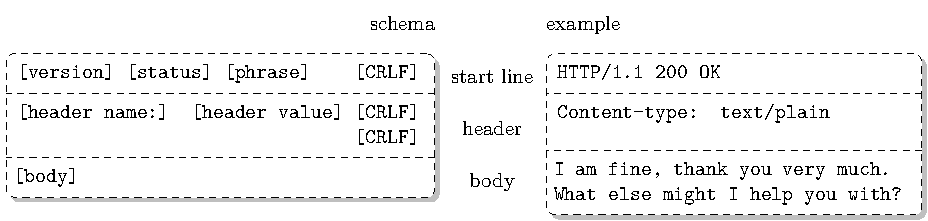
\includegraphics{fig/httpresponse.pdf}

\end{frame}

\begin{frame}[fragile]{getting the texts}

\begin{Shaded}
\begin{Highlighting}[]
\NormalTok{dominic <-}\StringTok{ }\KeywordTok{read_html}\NormalTok{(}\StringTok{"http://www.r-datacollection.com/blog/Fifty-years-of-Christmas-at-the-Windsors/"}\NormalTok{)}
\NormalTok{dominic <-}\StringTok{ }\KeywordTok{html_nodes}\NormalTok{(dominic, }\DataTypeTok{xpath=}\StringTok{"//p"}\NormalTok{)}
\NormalTok{dominic <-}\StringTok{ }\KeywordTok{html_text}\NormalTok{(dominic)}
\NormalTok{dominic <-}\StringTok{ }\KeywordTok{str_c}\NormalTok{(dominic, }\DataTypeTok{collapse=}\StringTok{"}\CharTok{\textbackslash{}n}\StringTok{"}\NormalTok{)}
\end{Highlighting}
\end{Shaded}

\end{frame}

\begin{frame}[fragile]{getting the texts}

\begin{Shaded}
\begin{Highlighting}[]
\NormalTok{peter <-}\StringTok{ }\KeywordTok{read_html}\NormalTok{(}\StringTok{"http://www.r-datacollection.com/blog/Introduction-to-Public-Attention-Analytics-with-Wikipediatrend/"}\NormalTok{)}
\NormalTok{peter <-}\StringTok{ }\KeywordTok{html_nodes}\NormalTok{(peter, }\DataTypeTok{xpath=}\StringTok{"//p"}\NormalTok{)}
\NormalTok{peter <-}\StringTok{ }\KeywordTok{html_text}\NormalTok{(peter)}
\NormalTok{peter <-}\StringTok{ }\KeywordTok{str_c}\NormalTok{(peter, }\DataTypeTok{collapse=}\StringTok{"}\CharTok{\textbackslash{}n}\StringTok{"}\NormalTok{)}
\end{Highlighting}
\end{Shaded}

\end{frame}

\begin{frame}[fragile]{getting the texts}

\begin{Shaded}
\begin{Highlighting}[]
\NormalTok{simon <-}\StringTok{ }\KeywordTok{read_html}\NormalTok{(}\StringTok{"http://www.r-datacollection.com/blog/Programming-a-Twitter-bot/"}\NormalTok{)}
\NormalTok{simon <-}\StringTok{ }\KeywordTok{html_nodes}\NormalTok{(simon, }\DataTypeTok{xpath=}\StringTok{"//p"}\NormalTok{)}
\NormalTok{simon <-}\StringTok{ }\KeywordTok{html_text}\NormalTok{(simon)}
\NormalTok{simon <-}\StringTok{ }\KeywordTok{str_c}\NormalTok{(simon, }\DataTypeTok{collapse=}\StringTok{"}\CharTok{\textbackslash{}n}\StringTok{"}\NormalTok{)}
\end{Highlighting}
\end{Shaded}

\end{frame}

\begin{frame}[fragile]{getting the texts}

\begin{Shaded}
\begin{Highlighting}[]
\NormalTok{christian <-}\StringTok{ }\KeywordTok{read_html}\NormalTok{(}\StringTok{"http://www.r-datacollection.com/blog/Hassle-free-data-from-HTML-tables-with-the-htmltable-package/"}\NormalTok{)}
\NormalTok{christian <-}\StringTok{ }\KeywordTok{html_nodes}\NormalTok{(christian, }\DataTypeTok{xpath=}\StringTok{"//p"}\NormalTok{)}
\NormalTok{christian <-}\StringTok{ }\KeywordTok{html_text}\NormalTok{(christian)}
\NormalTok{christian <-}\StringTok{ }\KeywordTok{str_c}\NormalTok{(christian, }\DataTypeTok{collapse=}\StringTok{"}\CharTok{\textbackslash{}n}\StringTok{"}\NormalTok{)}
\end{Highlighting}
\end{Shaded}

\end{frame}

\begin{frame}[fragile]{posting texts}

\begin{Shaded}
\begin{Highlighting}[]
\NormalTok{force <-}\StringTok{ }\NormalTok{F }\CommentTok{# redo or not}
\NormalTok{if ( !}\KeywordTok{file.exists}\NormalTok{(}\StringTok{"dominic.html"}\NormalTok{) |}\StringTok{ }\NormalTok{force==T)\{}
  \NormalTok{resp_d <-}\StringTok{ }\KeywordTok{POST}\NormalTok{(}\StringTok{"http://read-able.com/check.php"}\NormalTok{,}
            \DataTypeTok{body=}\KeywordTok{list}\NormalTok{(}\DataTypeTok{directInput=}\NormalTok{dominic), }
            \DataTypeTok{encode=}\StringTok{"form"}\NormalTok{)}
  \KeywordTok{writeBin}\NormalTok{(}\KeywordTok{content}\NormalTok{(resp_d, }\StringTok{"raw"}\NormalTok{), }
           \DataTypeTok{con=}\StringTok{"dominic.html"} \NormalTok{, }\DataTypeTok{useBytes=}\NormalTok{T)}
\NormalTok{\}}
\end{Highlighting}
\end{Shaded}

\end{frame}

\begin{frame}[fragile]{posting texts}

\begin{Shaded}
\begin{Highlighting}[]
\NormalTok{if ( !}\KeywordTok{file.exists}\NormalTok{(}\StringTok{"peter.html"}\NormalTok{)  |}\StringTok{ }\NormalTok{force==T)\{}
  \NormalTok{resp_p <-}\StringTok{ }\KeywordTok{POST}\NormalTok{(}\StringTok{"http://read-able.com/check.php"}\NormalTok{,}
            \DataTypeTok{body=}\KeywordTok{list}\NormalTok{(}\DataTypeTok{directInput=}\NormalTok{peter), }
            \DataTypeTok{encode=}\StringTok{"form"}\NormalTok{)}
  \KeywordTok{writeBin}\NormalTok{(}\KeywordTok{content}\NormalTok{(resp_p, }\StringTok{"raw"}\NormalTok{), }
           \DataTypeTok{con=}\StringTok{"peter.html"} \NormalTok{, }\DataTypeTok{useBytes=}\NormalTok{T)}
\NormalTok{\}}
\end{Highlighting}
\end{Shaded}

\end{frame}

\begin{frame}[fragile]{posting texts}

\begin{Shaded}
\begin{Highlighting}[]
\NormalTok{if ( !}\KeywordTok{file.exists}\NormalTok{(}\StringTok{"simon.html"}\NormalTok{) |}\StringTok{ }\NormalTok{force==T )\{}
  \NormalTok{resp_s <-}\StringTok{ }\KeywordTok{POST}\NormalTok{(}\StringTok{"http://read-able.com/check.php"}\NormalTok{,}
            \DataTypeTok{body=}\KeywordTok{list}\NormalTok{(}\DataTypeTok{directInput=}\NormalTok{simon), }
            \DataTypeTok{encode=}\StringTok{"form"}\NormalTok{)}
  \KeywordTok{writeBin}\NormalTok{(}\KeywordTok{content}\NormalTok{(resp_s, }\StringTok{"raw"}\NormalTok{), }
           \DataTypeTok{con=}\StringTok{"simon.html"} \NormalTok{, }\DataTypeTok{useBytes=}\NormalTok{T)}
\NormalTok{\}}
\end{Highlighting}
\end{Shaded}

\end{frame}

\begin{frame}[fragile]{posting texts}

\begin{Shaded}
\begin{Highlighting}[]
\NormalTok{if ( !}\KeywordTok{file.exists}\NormalTok{(}\StringTok{"christian.html"}\NormalTok{)  |}\StringTok{ }\NormalTok{force==T)\{}
  \NormalTok{resp_c <-}\StringTok{ }\KeywordTok{POST}\NormalTok{(}\StringTok{"http://read-able.com/check.php"}\NormalTok{,}
            \DataTypeTok{body=}\KeywordTok{list}\NormalTok{(}\DataTypeTok{directInput=}\NormalTok{christian), }
            \DataTypeTok{encode=}\StringTok{"form"}\NormalTok{)}
  \KeywordTok{writeBin}\NormalTok{(}\KeywordTok{content}\NormalTok{(resp_c, }\StringTok{"raw"}\NormalTok{), }
           \DataTypeTok{con=}\StringTok{"christian.html"} \NormalTok{, }\DataTypeTok{useBytes=}\NormalTok{T)}
\NormalTok{\}}
\end{Highlighting}
\end{Shaded}

\end{frame}

\begin{frame}[fragile]{the verdict}

\begin{Shaded}
\begin{Highlighting}[]
\NormalTok{verdict <-}\StringTok{ }\NormalTok{function(file)\{}
  \KeywordTok{read_html}\NormalTok{(file) %>%}\StringTok{ }
\StringTok{    }\KeywordTok{html_table}\NormalTok{() %>%}\StringTok{ }
\StringTok{    }\NormalTok{magrittr::}\KeywordTok{extract2}\NormalTok{(}\DecValTok{1}\NormalTok{) %>%}\StringTok{ }
\StringTok{    }\NormalTok{magrittr::}\KeywordTok{extract}\NormalTok{(}\DecValTok{2}\NormalTok{,)}
\NormalTok{\}}
\end{Highlighting}
\end{Shaded}

\end{frame}

\begin{frame}[fragile]{the verdict}

\begin{Shaded}
\begin{Highlighting}[]
\KeywordTok{verdict}\NormalTok{(}\StringTok{"simon.html"}\NormalTok{)}
\end{Highlighting}
\end{Shaded}

\begin{verbatim}
##                           X1  X2 X3
## 2 Flesch Kincaid Grade Level 7.4 NA
\end{verbatim}

\begin{Shaded}
\begin{Highlighting}[]
\KeywordTok{verdict}\NormalTok{(}\StringTok{"dominic.html"}\NormalTok{)}
\end{Highlighting}
\end{Shaded}

\begin{verbatim}
##                           X1  X2 X3
## 2 Flesch Kincaid Grade Level 8.1 NA
\end{verbatim}

\begin{Shaded}
\begin{Highlighting}[]
\KeywordTok{verdict}\NormalTok{(}\StringTok{"peter.html"}\NormalTok{)}
\end{Highlighting}
\end{Shaded}

\begin{verbatim}
##                           X1   X2 X3
## 2 Flesch Kincaid Grade Level 10.6 NA
\end{verbatim}

\begin{Shaded}
\begin{Highlighting}[]
\KeywordTok{verdict}\NormalTok{(}\StringTok{"christian.html"}\NormalTok{)}
\end{Highlighting}
\end{Shaded}

\begin{verbatim}
##                           X1 X2 X3
## 2 Flesch Kincaid Grade Level 11 NA
\end{verbatim}

\end{frame}

\section{GET and POST within Developer
Tools}\label{get-and-post-within-developer-tools}

\begin{frame}{GET and POST within Developer Tools}

Libve Clicking

\end{frame}

\end{document}
